\section{Supervisor}

\frame{\tableofcontents[currentsection]}

\begin{frame}
    \frametitle{Fundamentals of an exception}
    What is an exception?
     \begin{itemize}
         \item Exceptional behaviour that is abnormal
         \item Causes the current operation / process to crash
     \end{itemize}

     \vfill
     
     Examples
     \begin{itemize}
         \item HTTP request
         \item DB: Record locking (during insert)
     \end{itemize}
\end{frame}

% No added value of a slide of the demerits and then the merits. 
% Immediately talk about the merits

\begin{frame}
    \frametitle{Let it crash}
    \begin{itemize}
         \item Fail fast
         \item Only write code for the happy path
         \item Failures are completely isolated
         \item With try/catch, what about abnormal states?
         \item Restarting is often quicker than huge try/catch blocks
    \end{itemize}
    
    \vfill

    \tiny 
    Excellent 
    \href{https://elixirforum.com/t/understanding-the-advantages-of-let-it-crash-term/9748/19?u=wfransen}{forum post} 
    from Sasa Juric and a     
    \href{https://elixirforum.com/t/understanding-the-advantages-of-let-it-crash-term/9748/21?u=wfransen}{video}
    from Joe Armstrong 
\end{frame}


\begin{frame}
    \frametitle{Application-level supervisor}
    \begin{itemize}
        \item 99.999999\% uptime
        \item Autogenerated with the -sup option
    \end{itemize}
\end{frame}

\begin{frame}
    \frametitle{Goal}
    \begin{itemize}
        \item Process which supervises processes
        \item Supervision tree
        \item Fault-tolerance
    \end{itemize}
    \vfill
    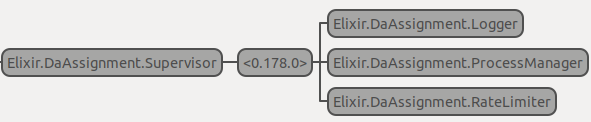
\includegraphics[scale=0.50]{01_supervision_tree}
\end{frame}

\begin{frame}
    \frametitle{Structure}
    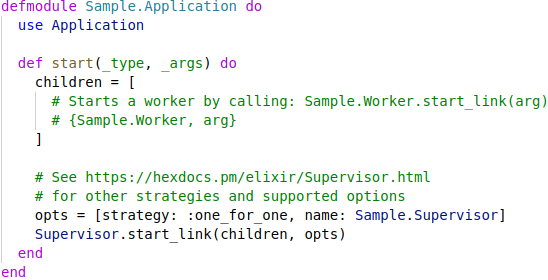
\includegraphics[scale=0.55]{02_application_sup}
\end{frame}

\begin{frame}
    \frametitle{Necessary information}
    \begin{itemize}
        \item How it should start the child.
        \item What it should do when the child terminates.
        \item How it should uniquely distinguish the child.
    \end{itemize}
    
    \vfill

    \footnotesize
    child specifications and supervisor restart strategy contains this information.
\end{frame}